\documentclass[aspectratio=169,11pt]{beamer}
\usepackage{teaching_slides}


\begin{document}

\title[Econometrics I]{ Econometrics I}
\subtitle{Bonus: How I work?}
\author{Chris Conlon \\NYU Stern}
\date{Fall 2026}
\maketitle

\begin{frame}{Final Thoughts}
Since this is a class about \alert{research methodology} it might be worthwhile to review what my workflow looks like:

\begin{itemize}
	\item There are lots of ways to organize your econometric analysis
	\item This is just the way that I do things
\end{itemize}
\end{frame}


\begin{frame}{My Computer}
\begin{itemize}
	\item I use mostly very standard Mac hardware ( a Macbook Air and a Mac Mini )
	\begin{itemize}
		\item You will be fine with a PC, but I like the Mac's UNIX filesystem and command line.
	\end{itemize}
	\item If I need something more than that, I use NYU's HPC cluster, now called \alert{Torch} (it replaced Greene):
	\url{https://services.rt.nyu.edu/docs/hpc/getting_started/intro/}
	\item I write mostly Python using VS Code \url{https://code.visualstudio.com}
	\item I use \alert{Claude Code} inside VS Code as a coding assistant
	\begin{itemize}
		\item Great for debugging, refactoring, plots/tables, and learning unfamiliar packages.
		\item You are still responsible for every number: read the code it writes, and ask it to show you checks.
	\end{itemize}
	\item I don't recommend using \texttt{conda} or \texttt{pip} for managing Python, I recommend using \texttt{uv} instead.
	\item I rarely download software from the web, when I can install it in \texttt{homebrew} \url{https://brew.sh}
	\begin{itemize}
		\item When I mean everything, I mean everything (R, Rstudio, Github, Spotify, LaTeX)
		\item Also for missing libraries that \texttt{R} links to.
	\end{itemize}
\end{itemize}
\end{frame}



\begin{frame}{Version Control}
You need to use it!
\begin{itemize}
	\item You will probably ignore this advice until something goes horribly wrong.
	\item Your projects should probably live in a \alert{private} GitHub repository.
	\item If GitHub is annoying you can use the Github Desktop interface \url{https://desktop.github.com/download/}.
	\item At the very least use Dropbox and pay for the \alert{extended history}
	\begin{itemize}
		\item But putting Github and Dropbox on the same folder will lead to disaster !
	\end{itemize}
	\item You will want to roll back to an older version more than you think!
	\item You will want to know exactly what changes your coauthor made all of the time!
\end{itemize}
\end{frame}



\begin{frame}{Organizing Projects}
\begin{columns}
\begin{column}{0.5\textwidth}
\begin{itemize}
	\item Always separate \alert{code} from \alert{data}
	\item Further separate code which \alert{processes data} from code which \alert{analyzes data}.
	\item Ultimately you will need a single script that runs the entire analysis from start to finish
	\item Start with a folder of \alert{raw data} and a folder of \alert{processed data}.
	\begin{itemize}
		\item Include directions on exactly where to get the data and \alert{appropriate citations} (including DOI).
	\end{itemize}
\end{itemize}
\end{column}
\begin{column}{0.5\textwidth}
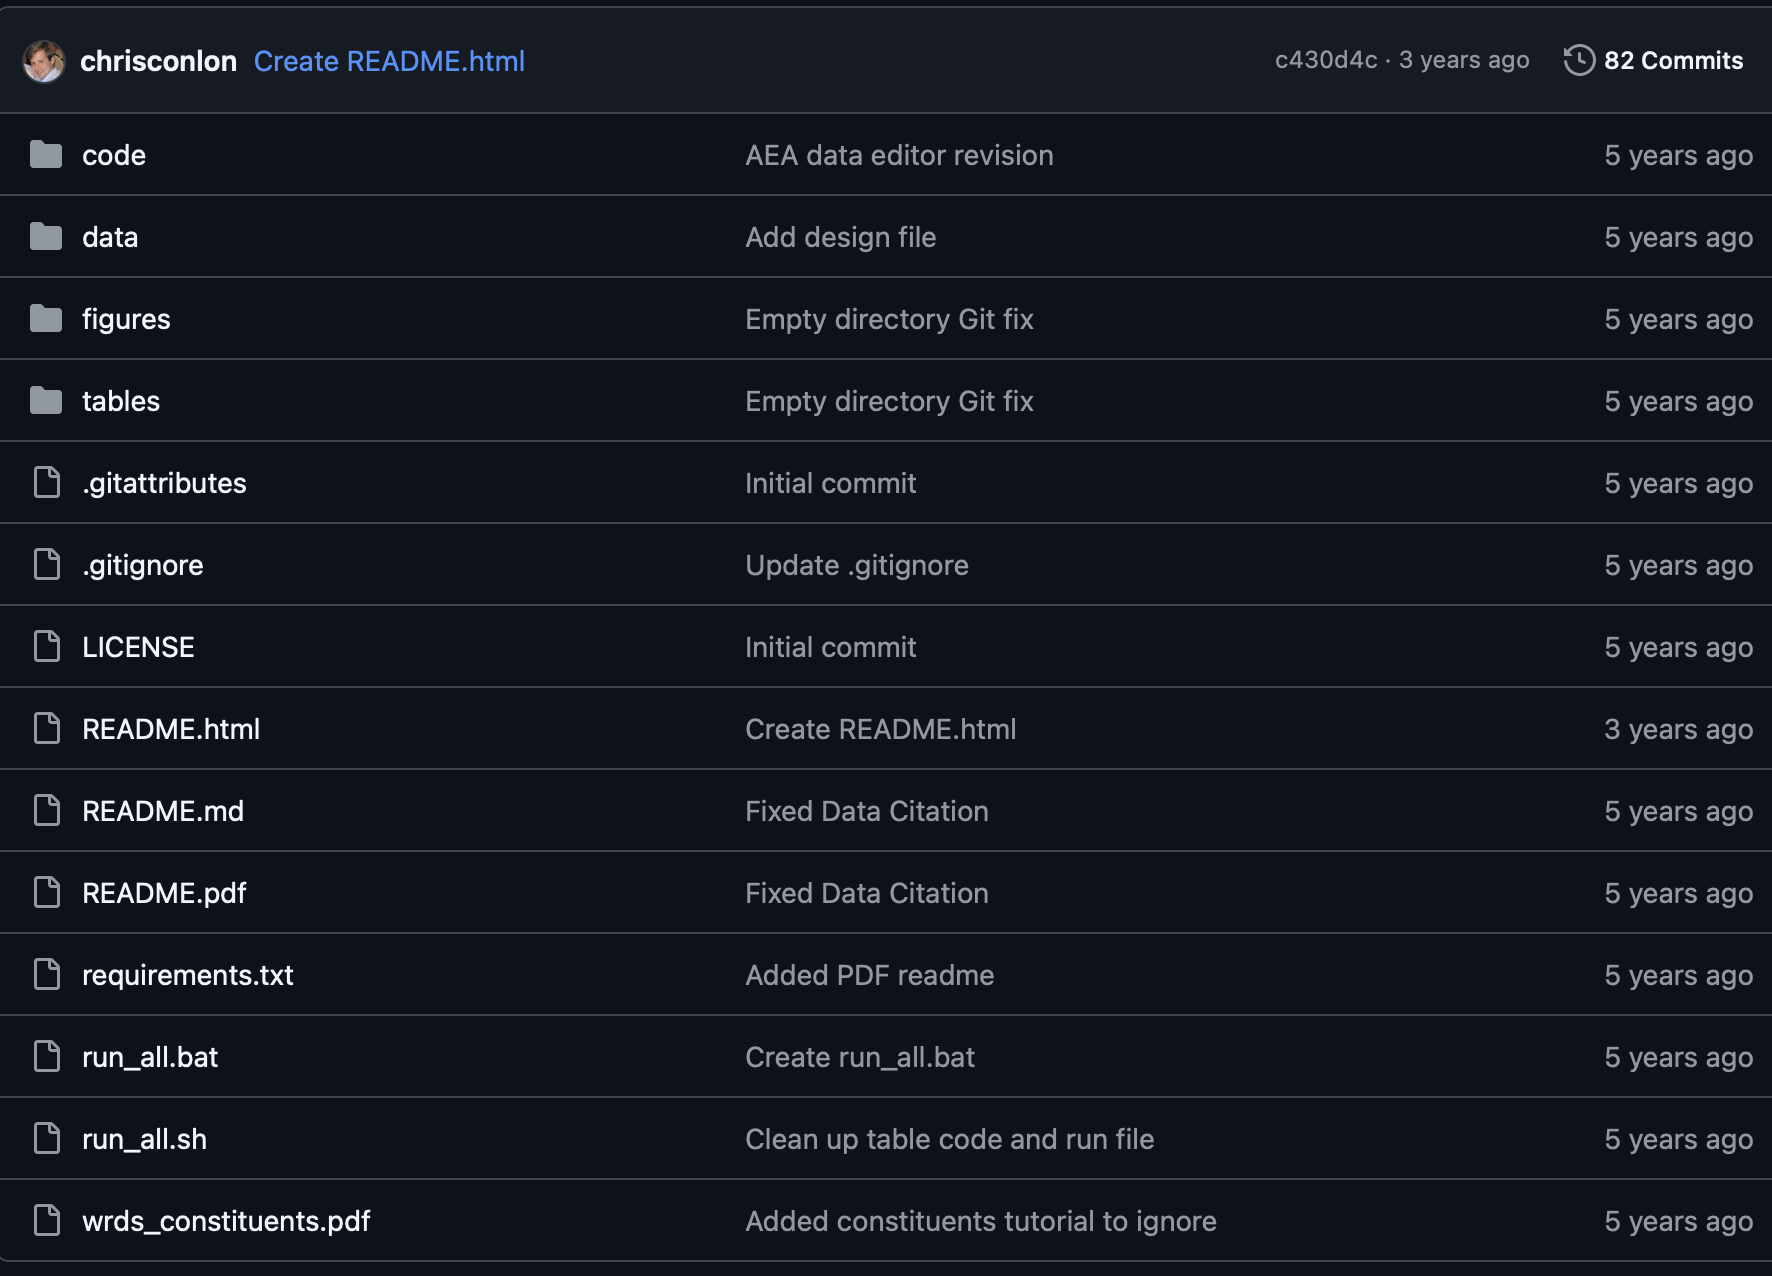
\includegraphics[width=\textwidth]{resources/co_replication1.png}
\end{column}
\end{columns}
\end{frame}


\begin{frame}{Organizing Projects}
\begin{columns}
\begin{column}{0.5\textwidth}
\begin{itemize}
	\item Number your files
	\item Try to avoid mixing cleaning/filtering data with \alert{analysis}, so that \alert{all analysis starts from a common dataset} with minimal processing.
	\begin{itemize}
		\item Otherwise you end up with red flags like tables with different numbers of observations (!)
	\end{itemize}\end{itemize}
	Let's take a look at \url{https://github.com/chrisconlon/CommonOwnerReplication}
\end{column}
\begin{column}{0.5\textwidth}
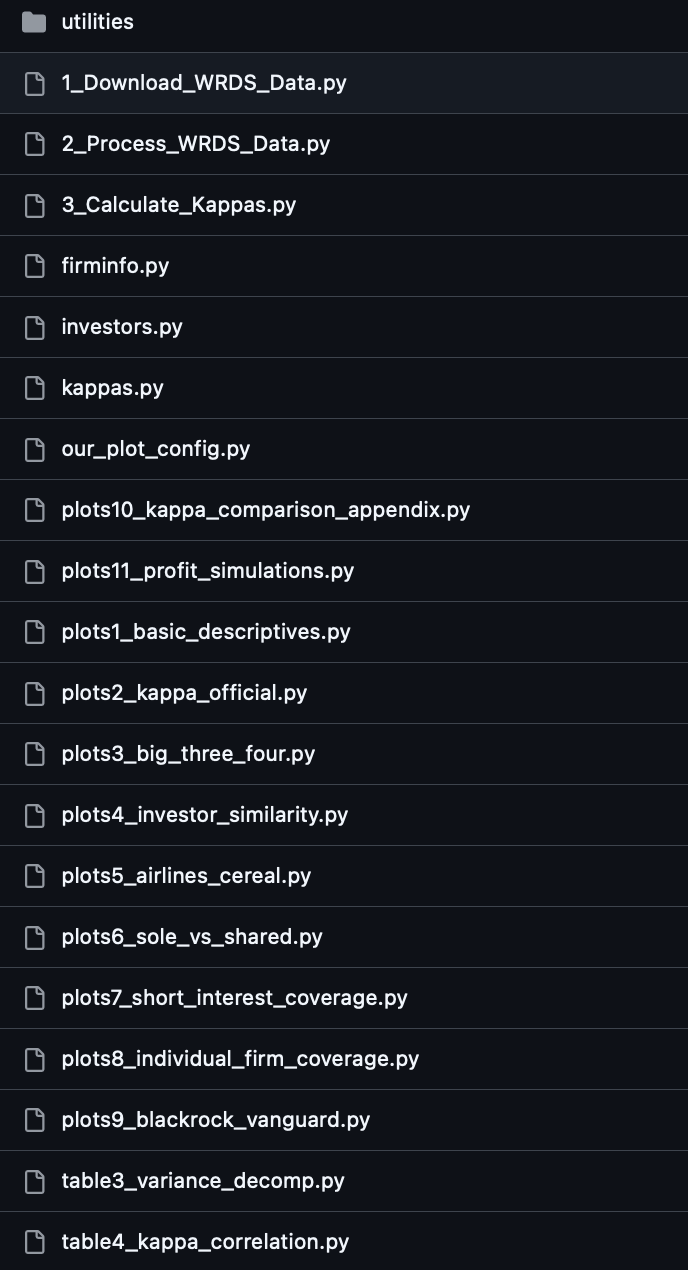
\includegraphics[width=0.7\textwidth]{resources/co_replication2.png}
\end{column}
\end{columns}
\end{frame}



\begin{frame}{Write Good Code}
Good Code has 
\begin{itemize}
	\item Clear Comment describing what the file does
	\item A list of all required \alert{inputs} and \alert{outputs}
	\item Detailed comments whenever you merge/drop observations
	\begin{itemize}
		\item Write separate checks to go through missings/drops/etc.
		\item I often just write them to an Excel file (!) to flip through more easily.
	\end{itemize}
	\item Shared routines and complicated logic can live in a separate file.
	\item Minimal side effects and dependencies.
\end{itemize}
\end{frame}


\begin{frame}{Avoid Bad Code}
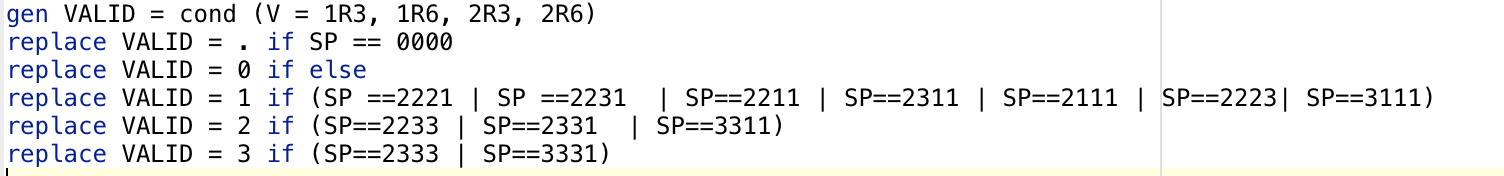
\includegraphics[width=0.95\textwidth]{resources/stata_disaster.png}
\begin{itemize}
	\item Big Blocks of ``Replace IF'' should probably be a \texttt{.csv} file and a merge.
	\item If you can take a big block of changes/drops/etc and make it \alert{data} instead of a code block, do that!
	\item This is easier to modify/maintain and catch mistakes.
\end{itemize}
\end{frame}

\begin{frame}{Big Data}
You may find yourself starting at terabytes of \texttt{.csv.gz} files.
\begin{itemize}
	\item Goal: filer/drop the rows you don't need and save them to a \texttt{.parquet} as quickly as possible.
	\begin{itemize}
		\item These compress really well and load very fast.
	\end{itemize}
	\item You can save multiple \texttt{.parquet} files in one directory and treat them as a giant (larger than RAM) file.
	\item In python you can use \texttt{polars} instead of \texttt{pandas} to read files larger than memory.
	\item The industrial strength version is \texttt{arrow} which works for both \texttt{R} and \texttt{Python}.
	\begin{itemize}
		\item You can read parts of files and process them chunk by chunk.
		\item You can filter without loading the whole file
		\item And save directly to \texttt{.parquet}
	\end{itemize}
	\item NEVER USE \texttt{.RDATA} (you will thank me later).
\end{itemize}
See my project that ingests 2TB of data and saves about 1.5GB of cleaned data in <5min.
\end{frame}



\begin{frame}{Writing Papers}
You have some choices here
\begin{itemize}
	\item Most people use Overleaf for academic papers \url{www.overleaf.com} (which NYU subscribes to)
	\begin{itemize}
		\item The main feature is that multiple people can edit paper at once
		\item Otherwise you should use Github/ Version Control
	\end{itemize}
	\item You probably want a \LaTeX install on your computer just in case.
	\item Writing a paper in an environment without a spellcheck, etc. is insane (don't do this).
	\item Put your citations in a bibliography manager like \url{www.zotero.com} otherwise you will spend forever formatting and updating them.
	\item Don't worry too much about formatting paper/citations until paper is accepted, but you need them to be \alert{accurate} always.
	\item If you are really fancy you can sync all of the tables figures to update the paper automatically (this can lead to surprises).
\end{itemize}
\end{frame}

\section*{Thanks!}


\end{document}
